\documentclass[journal]{vgtc}                % final (journal style)
%\documentclass[review,journal]{vgtc}         % review (journal style)
%\documentclass[widereview]{vgtc}             % wide-spaced review
%\documentclass[preprint,journal]{vgtc}       % preprint (journal style)

%% Uncomment one of the lines above depending on where your paper is
%% in the conference process. ``review'' and ``widereview'' are for review
%% submission, ``preprint'' is for pre-publication, and the final version
%% doesn't use a specific qualifier.

%% Please use one of the ``review'' options in combination with the
%% assigned online id (see below) ONLY if your paper uses a double blind
%% review process. Some conferences, like IEEE Vis and InfoVis, have NOT
%% in the past.

%% Please use the ``preprint''  option when producing a preprint version
%% for sharing your article on an open access repository

%% Please note that the use of figures other than the optional teaser is not permitted on the first page
%% of the journal version.  Figures should begin on the second page and be
%% in CMYK or Grey scale format, otherwise, colour shifting may occur
%% during the printing process.  Papers submitted with figures other than the optional teaser on the
%% first page will be refused. Also, the teaser figure should only have the
%% width of the abstract as the template enforces it.

%% These few lines make a distinction between latex and pdflatex calls and they
%% bring in essential packages for graphics and font handling.
%% Note that due to the \DeclareGraphicsExtensions{} call it is no longer necessary
%% to provide the the path and extension of a graphics file:
%% 
\includegraphics{diamondrule} is completely sufficient.
%%
\ifpdf%                                % if we use pdflatex
  \pdfoutput=1\relax                   % create PDFs from pdfLaTeX
  \pdfcompresslevel=9                  % PDF Compression
  \pdfoptionpdfminorversion=7          % create PDF 1.7
  \ExecuteOptions{pdftex}
  \usepackage{graphicx}                % allow us to embed graphics files
  \DeclareGraphicsExtensions{.pdf,.png,.jpg,.jpeg} % for pdflatex we expect .pdf, .png, or .jpg files
\else%                                 % else we use pure latex
  \ExecuteOptions{dvips}
  \usepackage{graphicx}                % allow us to embed graphics files
  \DeclareGraphicsExtensions{.eps}     % for pure latex we expect eps files
\fi%

%% it is recomended to use ``\autoref{sec:bla}'' instead of ``Fig.~\ref{sec:bla}''
\graphicspath{{figures/}{pictures/}{images/}{./}} % where to search for the images

\usepackage{microtype}                 % use micro-typography (slightly more compact, better to read)
\PassOptionsToPackage{warn}{textcomp}  % to address font issues with \textrightarrow
\usepackage{textcomp}                  % use better special symbols
\usepackage{mathptmx}                  % use matching math font
\usepackage{times}                     % we use Times as the main font
\renewcommand*\ttdefault{txtt}         % a nicer typewriter font
\usepackage{cite}
\usepackage{graphics}                      % needed to automatically sort the references                      % only used for the table example
\usepackage{booktabs}
\usepackage{float}
\graphicspath{{./figs/}}                 % only used for the table example
%% We encourage the use of mathptmx for consistent usage of times font
%% throughout the proceedings. However, if you encounter conflicts
%% with other math-related packages, you may want to disable it.

%% In preprint mode you may define your own headline. If not, the default IEEE copyright message will appear in preprint mode.
%\preprinttext{To appear in IEEE Transactions on Visualization and Computer Graphics.}

%% In preprint mode, this adds a link to the version of the paper on IEEEXplore
%% Uncomment this line when you produce a preprint version of the article 
%% after the article receives a DOI for the paper from IEEE
%\ieeedoi{xx.xxxx/TVCG.201x.xxxxxxx}

%% If you are submitting a paper to a conference for review with a double
%% blind reviewing process, please replace the value ``0'' below with your
%% OnlineID. Otherwise, you may safely leave it at ``0''.
\onlineid{0}

%% declare the category of your paper, only shown in review mode
\vgtccategory{Research}
%% please declare the paper type of your paper to help reviewers, only shown in review mode
%% choices:
%% * algorithm/technique
%% * application/design study
%% * evaluation
%% * system
%% * theory/model
\vgtcpapertype{please specify}

%% Paper title.
\title{CS594 - Big Data Visualization \& Analytics: Proposal}

%% This is how authors are specified in the journal style

%% indicate IEEE Member or Student Member in form indicated below
\author{Ashwin Bhaskar Srivatsa, Sasanka Mouli Veleti  and Sidharth Veluvolu}
\authorfooter{
	%% insert punctuation at end of each item
	\item
	Ashwin Bhaskar Srivatsa, E-mail: asriva36@uic.edu
	\item
	Sasanka Mouli Veleti, E-mail: svelet2@uic.edu
	\item
	Sidharth Veluvolu, Email: sveluv2@uic.edu
}

%other entries to be set up for journal
\shortauthortitle{Biv \MakeLowercase{\textit{et al.}}: Global Illumination for Fun and Profit}
%\shortauthortitle{Firstauthor \MakeLowercase{\textit{et al.}}: Paper Title}

%% Abstract section.
%\abstract{Duis autem vel eum iriure dolor in hendrerit in vulputate
%velit esse molestie consequat, vel illum dolore eu feugiat nulla
%facilisis at vero eros et accumsan et iusto odio dignissim qui blandit
%praesent luptatum zzril delenit augue duis dolore te feugait nulla
%facilisi. Lorem ipsum dolor sit amet, consectetuer adipiscing elit,
%sed diam nonummy nibh euismod tincidunt ut laoreet dolore magna
%aliquam erat volutpat. Ut wisi enim ad minim veniam, quis nostrud exerci tation ullamcorper
%suscipit lobortis nisl ut aliquip ex ea commodo consequat. Duis autem
%vel eum iriure dolor in hendrerit in vulputate velit esse molestie
%consequat, vel illum dolore eu feugiat nulla facilisis at vero eros et
%accumsan et iusto odio dignissim qui blandit praesent luptatum zzril
%delenit augue duis dolore te feugait nulla facilisi.%
%} % end of abstract

%% Keywords that describe your work. Will show as 'Index Terms' in journal
%% please capitalize first letter and insert punctuation after last keyword
%% \keywords{Radiosity, global illumination, constant time}

%% ACM Computing Classification System (CCS). 
%% See <http://www.acm.org/class/1998/> for details.
%% The ``\CCScat'' command takes four arguments.

%% \CCScatlist{ % not used in journal version
%% \CCScat{K.6.1}{Management of Computing and Information Systems}%
%% {Project and People Management}{Life Cycle};
%% \CCScat{K.7.m}{The Computing Profession}{Miscellaneous}{Ethics}
%% }

%% A teaser figure can be included as follows
%\teaser{
%  \centering
%  \includegraphics[width=\linewidth]{CypressView}
%  \caption{In the Clouds: Vancouver from Cypress Mountain. Note that the teaser may not be wider than the abstract block.}
%  \label{fig:teaser}
%}

%% Uncomment below to disable the manuscript note
\renewcommand{\manuscriptnotetxt}{}

%% Copyright space is enabled by default as required by guidelines.
%% It is disabled by the 'review' option or via the following command:
% \nocopyrightspace


\vgtcinsertpkg

%%%%%%%%%%%%%%%%%%%%%%%%%%%%%%%%%%%%%%%%%%%%%%%%%%%%%%%%%%%%%%%%
%%%%%%%%%%%%%%%%%%%%%% START OF THE PAPER %%%%%%%%%%%%%%%%%%%%%%
%%%%%%%%%%%%%%%%%%%%%%%%%%%%%%%%%%%%%%%%%%%%%%%%%%%%%%%%%%%%%%%%%

\begin{document}

%% The ``\maketitle'' command must be the first command after the
%% ``\begin{document}'' command. It prepares and prints the title block.

%% the only exception to this rule is the \firstsection command


\maketitle


\section{Introduction}
Noise Pollution is a grievous problem which needs to be tackled, as it’s a growing concern for many urban residents, many have reported that they suffered with behavioral and emotional consequences, such as difficulty in sleeping, relaxing and feeling annoyed, angry or upset ~\cite{1} ~\cite{2} ~\cite{3}.In order to mitigate this problem, there is a need to understand sound event detection. Sound event detection is defined as recognition of individual sound events in audio, e.g., “dog barking, engine exhaust noise” requiring estimation of onset and offset for distinct sound for sound event detection and identification of sound.

 Applications for sound event detection can found in areas of Healthcare, security, audio and video-based indexing and retrieval. Sound class classification is usually approached as a supervised learning, with sound classes defined beforehand, we have taken a labelled Spatial and Temporal recording data which comprises of 3068 labelled 10 sec recordings from the Sounds of New York City (SONYC) acoustic network (An acoustic network is a method of positioning equipment using sound waves). Using this data, we plan to develop an application where the authorities or the user can narrow down the sounds generated at any particular location. We also aim to address the Mismatch of the testing data in this dataset.


This can be done by applying machine learning algorithm on any dataset and integrating it with sensors, data analytics for the development of machine learning systems for real world urban noise monitoring. The model build from the data could be used on neighborhoods to better understand noise in that location and help the authorities mitigate the issue. The many challenges for building the model would be like to separate the sound sources of interest, identifying the similar sounds compared to the other data in the dataset, identifying the main source for generating the sound among others.     

\section{Related work}
\section{Data description}
The dataset contains a training subset (13538 recordings from 35 sensors), and validation subset (4308 recordings from 9 sensors), and a test subset (669 recordings from 48 sensors). Each recording has been annotated using a set of 23 “tags” like “engine presence, machinery presence, non-machinery-impact presence, dog-barking-whining presence” ~\cite{4}.

The audio files used were recorded using the SONYC acoustic sensor network for monitoring urban noise pollution. In New York City, over 60 distinct sensors have been placed accumulating the equivalent of more than 50 years of audio data, of which a small fraction was used. The data was sampled by picking the closest neighbors based on VGGish qualities of recordings with recognized classes of interest. All of the recordings are 10 seconds long and were made with the same microphones and gain settings. 

The training, validation, and test subsets of the annotation data are contained in annotations.csv. Each row in the file represents one multi-label annotation of a recording—it might be a single citizen science volunteer's annotation, a single SONYC team member's annotation, or the SONYC team's agreed-upon ground truth (for more information, see the annotator id column description).

The sensors in the test set will not disjoint from the training and validation subsets, but the test recordings are displaced in time, occurring after any of the recordings in the training and validation subset. We plan to use the test data to find out the aggregate of mismatch by using a Multi Label classification Machine Learning Model

	
	\begin{figure}[h!]
		
		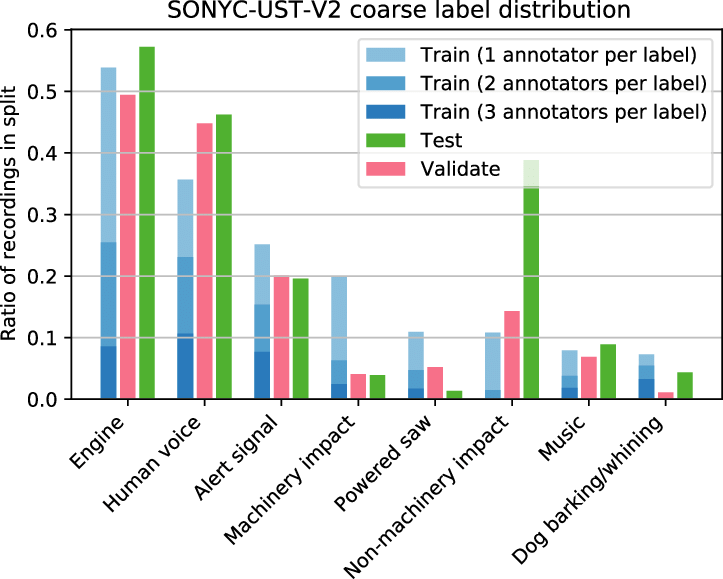
\includegraphics[width=9cm]{figure1}
		\caption{ Classes distibution in data}
	\end{figure}
	


	
	
	
	

	
	
	\section{Proposal}
    We propose to build a tool which would visualize the spatiotemporal values of the dataset, visuliaze the output of Machine Learning model and also visualize the points where the mismatches of testing and machine data occur based on the results of the Machine Learning model. We will be using Multi Label Classification Machine Learning Algorithms like support vector machines and existing neural networks to classify the audio files into various categorical sounds. Based on the results of ML model and mismatch plot, we would dwell into understanding the mismatches which occur between the annotated and machine predicted data and analyze the causes behind it. 
    
    The technologies which we plan to use in order to build this tool would be ReactJS on the front-end and Django on the back-end. We are using ReactJS because of its component based architecture and its rich support with D3.js, Open Layers. Similarly, Django allows us run various python libraries to process the data and creation of REST API's(representational state transfer application programming interface) to communicate with the front-end. 
   
   	We have divided the process of building this tool into four stages(see Figure 2) namely Data Preprocessing state wherein we process the audio files,Modeling stage where in Applying the Classification model on the dataset and creating REST API's to interact with the front-end, Visualization stage where in we visualize the results of machine learning model on the front-end, component building stage where we build components which allows the user to pick spatial and temporal values of various sound samples and display the results on a map.
   	
    The built tool would be useful to authorities who monitor sounds around the city would allow them to pinpoint the location of sound origin.
	\begin{figure}[h!]
	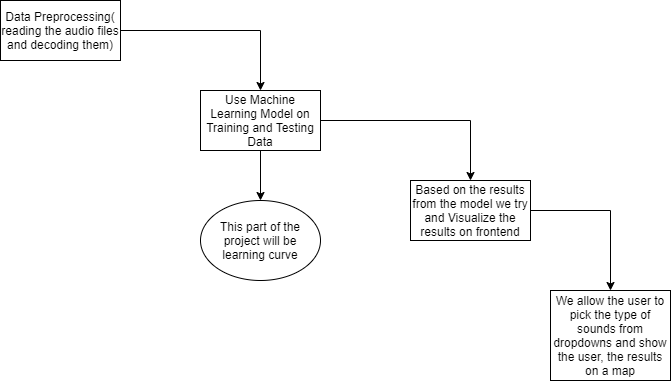
\includegraphics[width=9cm]{figure2}
	\caption{ Work flow diagram}
	\end{figure}
	
	

\section{Timeline} 

%\bibliographystyle{abbrv}
\bibliographystyle{abbrv-doi}
%\bibliographystyle{abbrv-doi-narrow}
%\bibliographystyle{abbrv-doi-hyperref}
%\bibliographystyle{abbrv-doi-hyperref-narrow}

\bibliography{proposal}
\end{document}
